\par Para este experimento evaluamos la red inalámbrica de los laboratorios del DC.

\subsubsection{Fuente $S$}

\par A continuación podemos ver la fuente $S$ propuesta modelada con los resultados del experimento: \\

\begin{tabular}{ | c | c | c |}
    \hline
    Mensaje & Probabilidad & Información [bits] \\
    \hline
    \textit{Unicast} & 0.773 & 0.371 \\
    \hline
    \textit{Broadcast} & 0.227 & 2.141 \\
    \hline
\end{tabular} \\

\par Entropía de la fuente: 0.772 bits. Entropía máxima: 1 bit.

\par Observamos que la entropía de la fuente es menor que la máxima, ya que las transmisiones \textit{unicast} son casi 3 veces más probables que las \textit{broadcast}.
Esto nos provee una cota inferior para el \textit{overhead} impuesto por los protocolos de control: al menos 22.7\% de los frames no transmiten datos.

\par Ya que no poseemos una idea del comportamiento esperado de esta fuente, no podemos realizar un análisis más detallado sólo a partir de esta fuente.
Por ende, lo profundizaremos recién en la sección del siguiente experimento, comparando con los resultados obtenidos de esa red.
%vemos que la entropía y la probabilidad de los frames \textit{broadcast} son significativamente mayores para la fuente $S$ en el experimento 2.

%\par Podemos ver, comparando la estructura de ambas redes (figuras \ref{ARPDC-sinColapsar} y \ref{ARPTrab-sinColapsar}, respectivamente), que la de este experimento es más fragmentaria, mientras que la del 2 posee un mucho mayor grado de interconexión.

\subsubsection{Fuente $S_1$}

\par En las figuras \ref{ARPDC-sinColapsar} y \ref{ARPDC} se pueden ver los grafos\footnote{Ambos grafos representan la misma red. Sin embargo, el tamaño del grafo \ref{ARPDC-sinColapsar} puede dificultar un análisis detallado, por lo que en la figura \ref{ARPDC} colapsamos ciertos nodos con iguales vecinos (que se muestran en rojo). Mantuvimos el grafo original ya que una mirada rápida ofrece más información concerniente a la topología de la red.} de la red subyacente de mensajes ARP.

\begin{figure*}[ht]
    \centering
    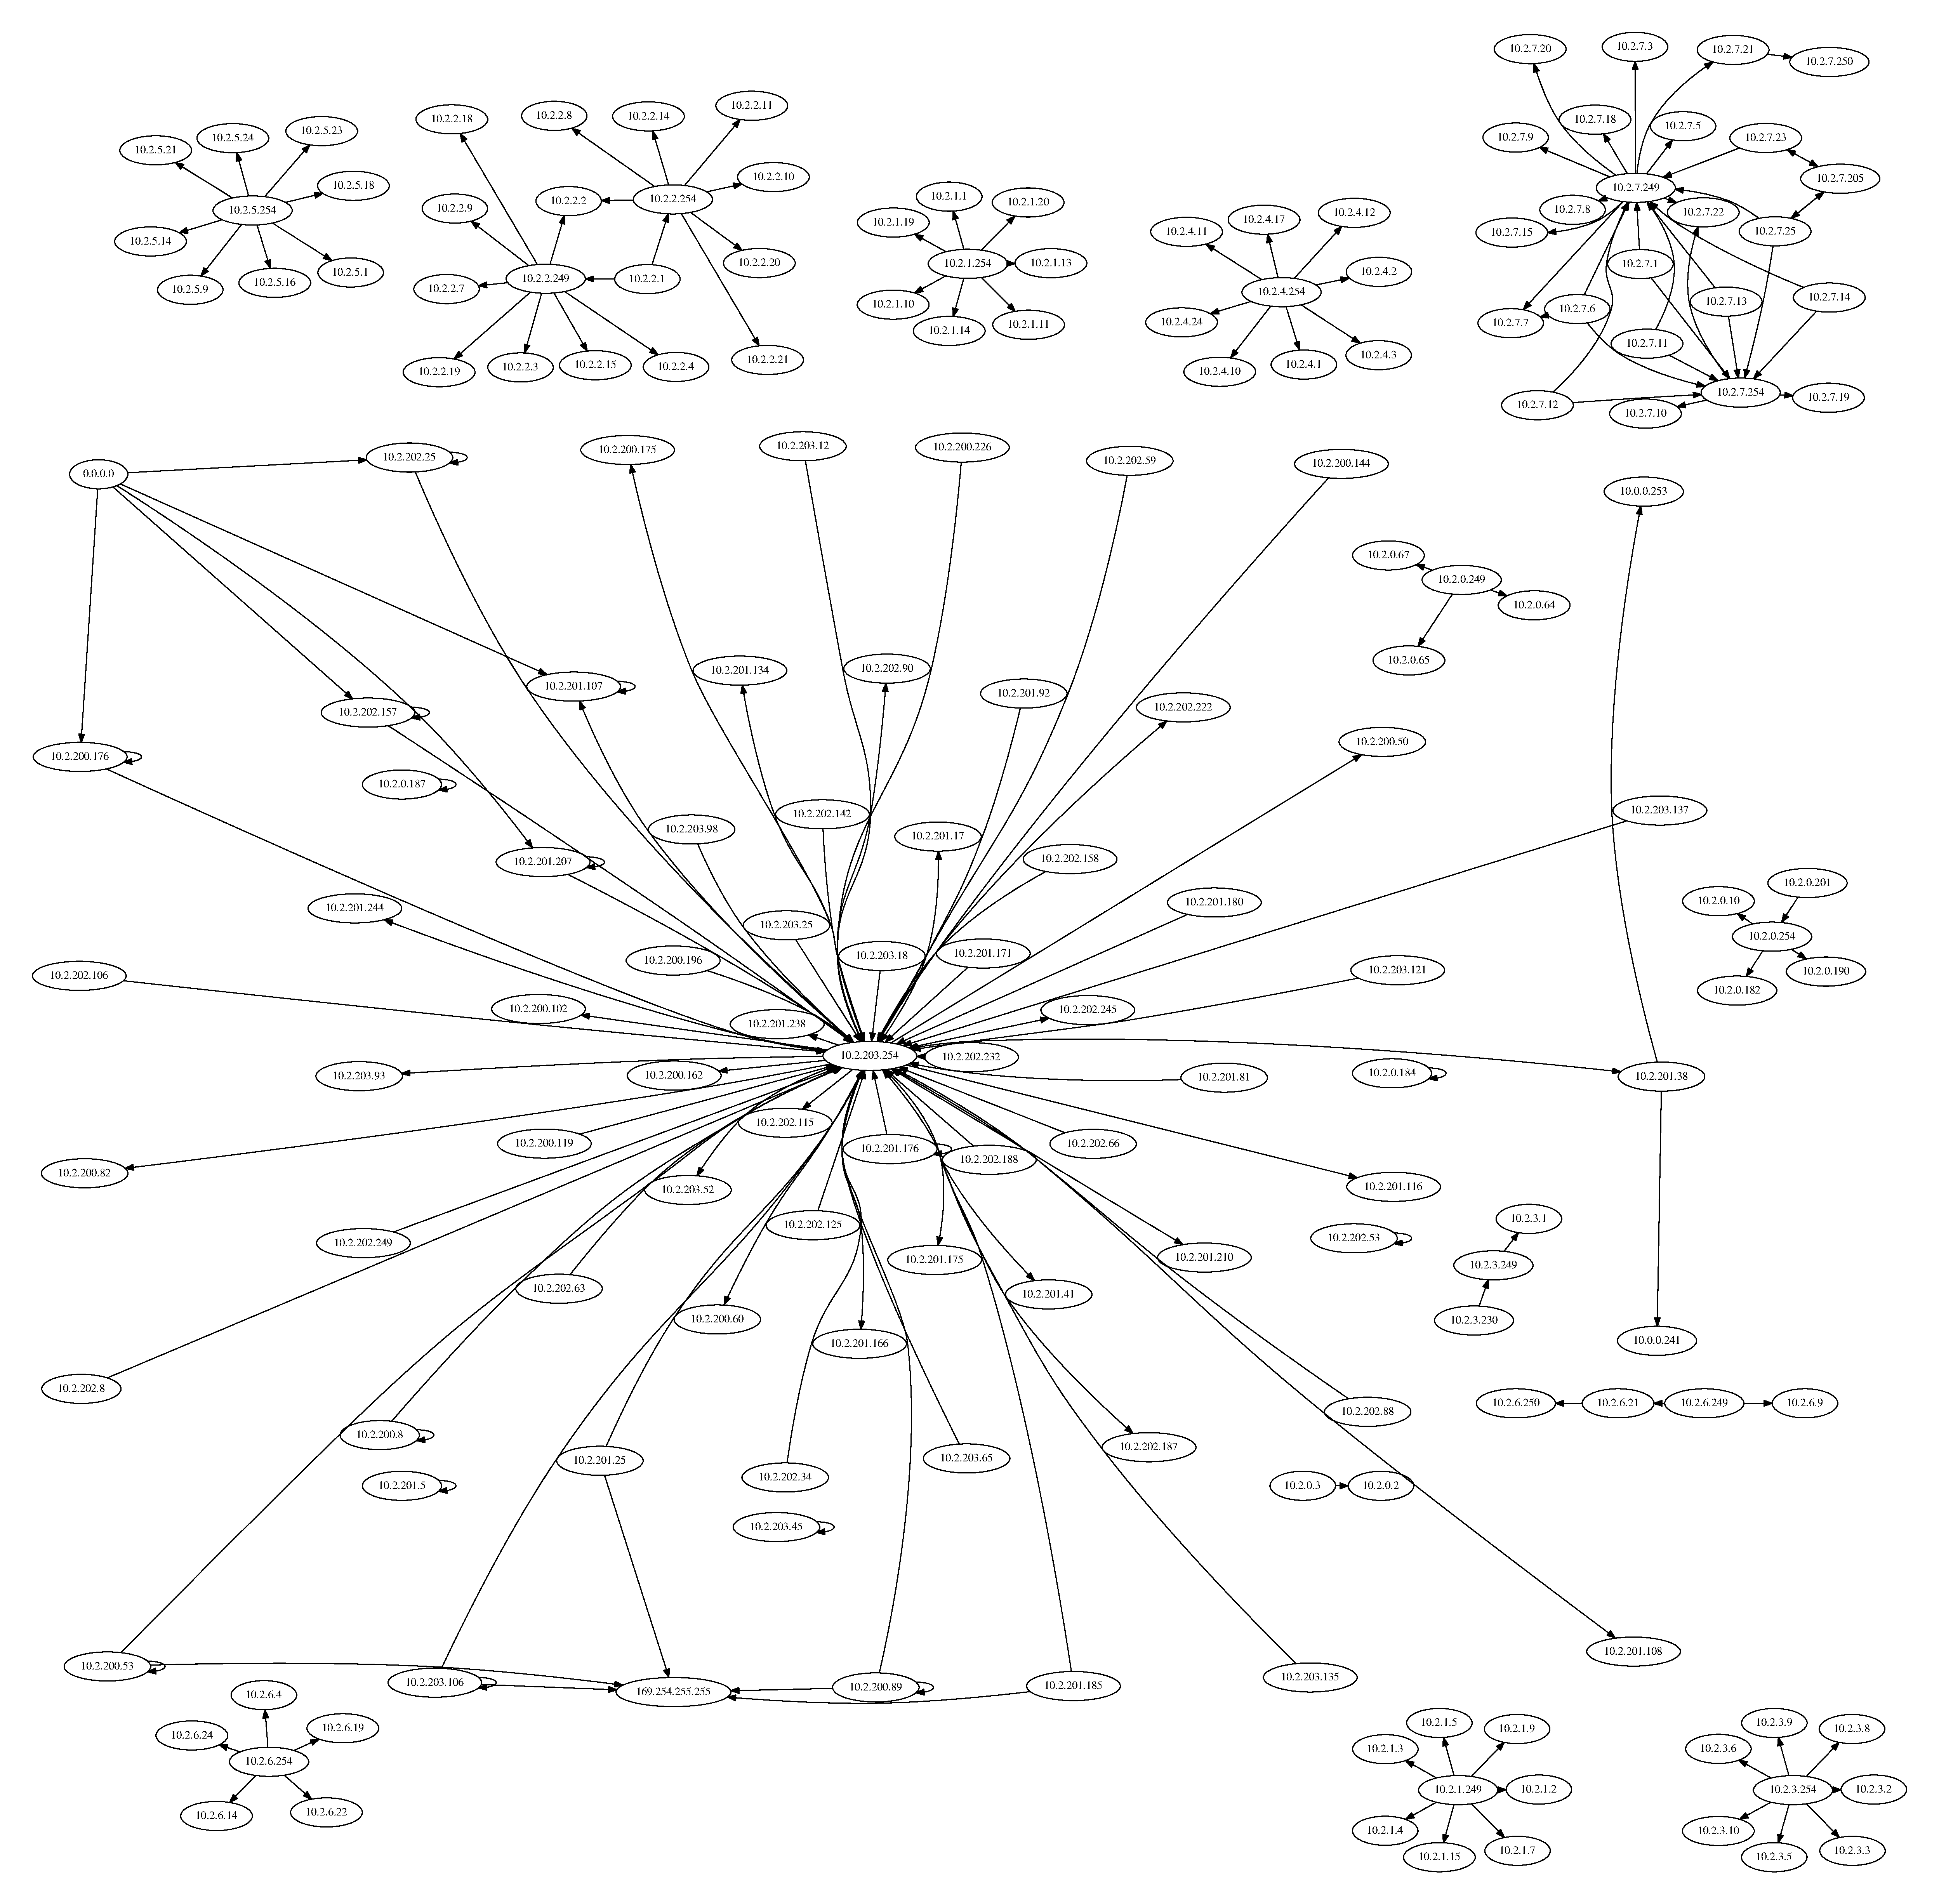
\includegraphics[width=0.9\textwidth]{figuras/ciudad_10_grafoSinColapsar.pdf}
    \caption{Grafo de la red subyacente de mensajes ARP, sin colapsar nodos .}\label{ARPDC-sinColapsar}
\end{figure*}

\begin{figure*}[ht]
    \centering
    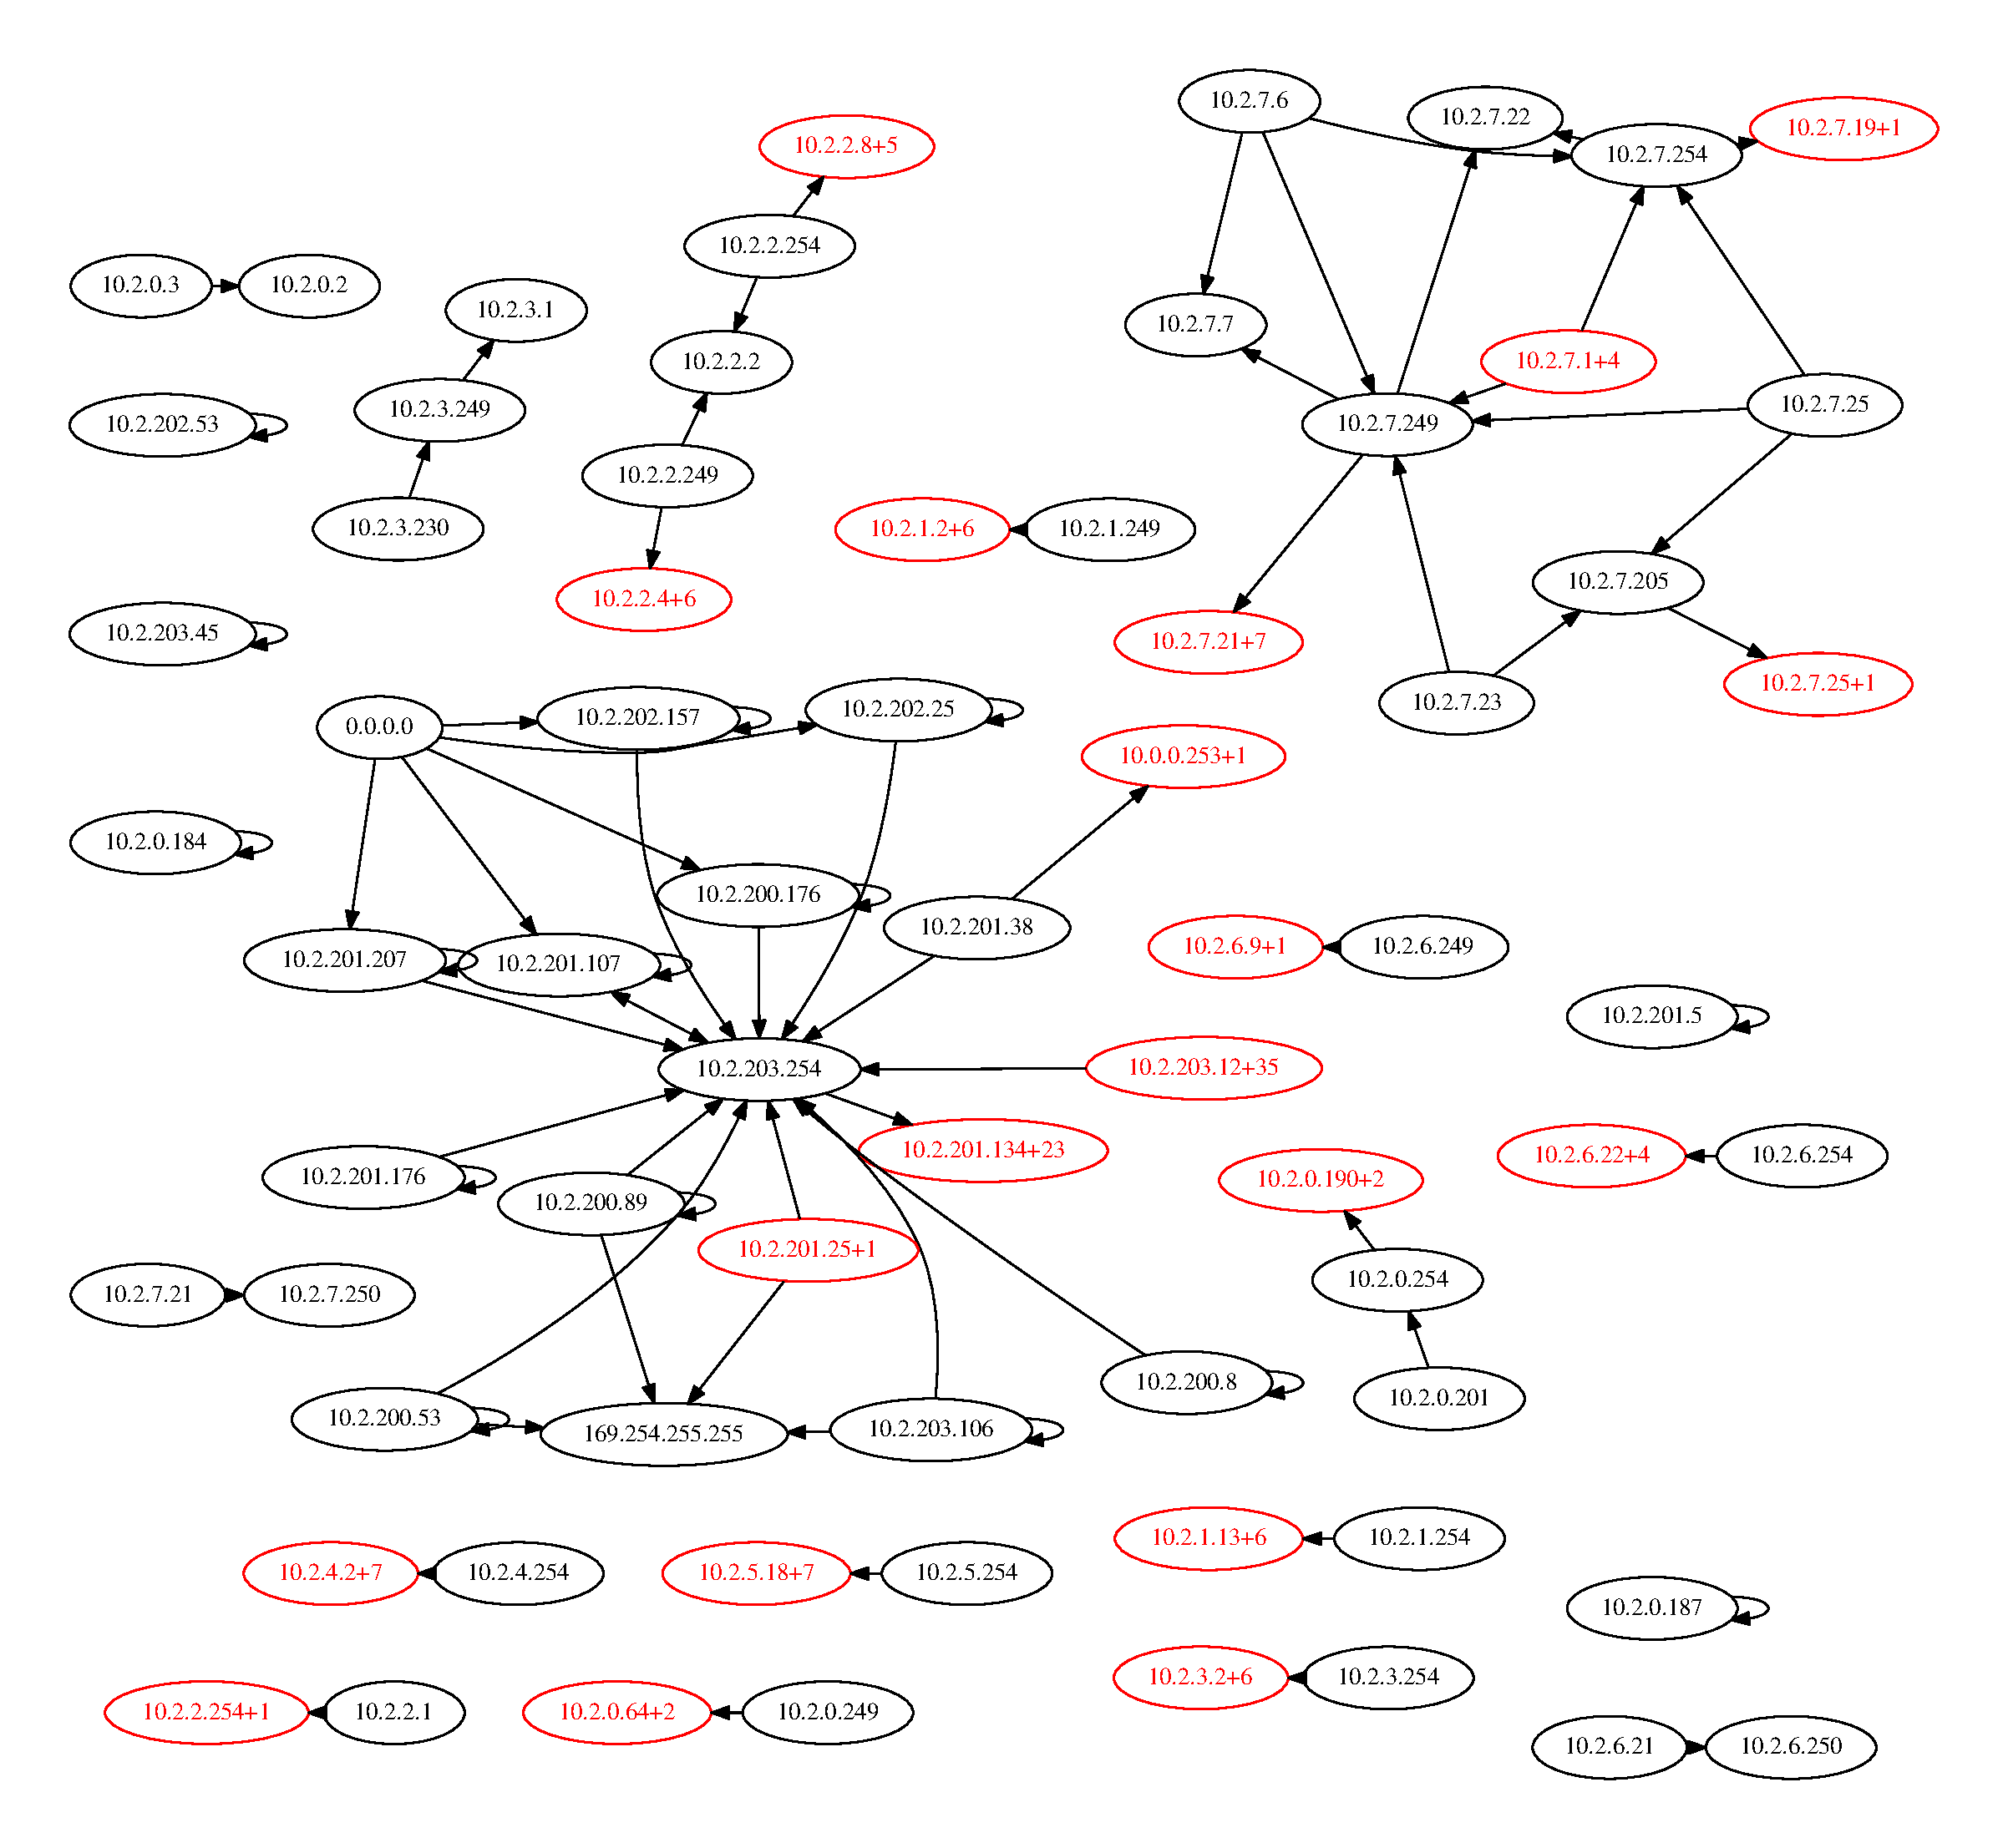
\includegraphics[width=0.9\textwidth]{figuras/ciudad_10_grafo.pdf}
    \caption{Grafo de la red subyacente de mensajes ARP, colapsando nodos.}\label{ARPDC}
\end{figure*}

\par Las direcciones IP de la red son de la forma 10.2.X.Y, con una sola excepción que mencionaremos más adelante.
Éstas son direcciones IP privadas\footnote{Todo el rango 10.0.0.0-10.255.255.255 es privado.}.

\par La red se presenta altamente fragmentada; el grafo posee múltiples componentes conexas.
Adicionalmente, vemos repetido un patrón entre varias de estas componentes: un nodo central, con una dirección IP de la forma 10.2.X.254 o 10.2.X.249, que envía paquetes a múltiples hojas\footnote{Se presenta una estructura de estrella, o cercana.}.
Esta estructura es consistente con el comportamiento esperado de Default Gateways. 

\par Hay un nodo claramente destacado en la red, el de dirección IP 10.2.203.254, que tanto envía como recibe paquetes de un gran número de hojas.

\par Se advierten diversas anomalías: en primer lugar, loops en el grafo, que como mencionamos previamente, se deben a \textit{gratuitous ARPs}; en segundo lugar, la dirección 0.0.0.0 se hace presente en el grafo, siempre como origen, lo que ejemplifica \textit{ARP probing}; finalmente, una única IP que no comienza con 10.2, la 169.254.255.255.
El rango 169.254.0.0-169.254.255.255 está reservado; se asigna cuando un dispositivo no tiene IP estática, y el protocolo dinámico\footnote{DHCP siendo actualmente el más común.} utilizado falla.

\begin{itemize}
	\item Dada la fuente S1, mostrar la cantidad de información de cada símbolo comparando con la entropía de la fuente.
\end{itemize}

Responder las siguientes preguntas (solo dejar las respuestas):

\begin{itemize}
	\item ¿Existe una correspondencia entre lo que se conoce de la red y los nodos distinguidos detectados por la herramienta? ¿Es posible usar el criterio de distinción propuesto como método para descubrir el/los Default Gateway/s de la red? ¿Es preciso?
\end{itemize}